\chapter{Basic principles of IPT}

This chapter will first introduce the principle of IPT technology from the physical level, and then introduce the principle of IPT technology from the circuit level, analyze the relationship between different equivalent models, and derive system energy transmission indicators that can represent system performance. And analyze the influence of relevant design parameters on system transmission performance. Analyze the influence of the medium on the system performance in the WPT process, and propose an equivalent model in the underwater working environment. Perform simulation analysis on the derivation to ensure that complete theoretical support is provided for more detailed theoretical research and research on new IPT technology.


\section{Inductive coupling model}
Figure \ref{WPT} depicts the circuit model of IPT systems, where the transmitting coil $L_1$ and the receiving coil $L_2$ are directly connected to the power source and the load, respectively. Denote $M$ as the mutual inductance, $r_1$ and $r_2$ as the equivalent AC resistance of coils.

\begin{figure}[!b]
    \centering
    \begin{tikzpicture}[scale=1, every node/.style={scale=1}, american voltages]
        \draw
        (0,3.5) to [R, l_=$r_1$, o-, f_=$I_p$, current arrow scale=24] (4,3.5)
        to [L, l=$L_1$] (4,0)
        to [short, -o] (0,0);
        \draw
        (6,3.5) to [L, l_=$L_2$, mirror] (6,0)
        to [short, -o] (10,0) ;
        \draw (10,3.5) to [R, l=$r_2$,o-, f=$I_s$, current arrow scale=24] (6,3.5);

        % source
        \node[below] at (5,3.5) {$M$};
        \draw [{<->}](4.234,2.6428) arc (139.9978:40:1);
        \draw [->,thick] (0,0.5) -- (0,3);
        \node[below] at (0.5,2) {$V_p$};
        \node[below] at (0.5,3) {+};
        \node[below] at (0.5,0.5) {–};

        \draw [->,thick] (10,0.5) -- (10,3);
        \node[below] at (10.5,2) {$V_s$};
        \node[below] at (9.5,3) {+};
        \node[below] at (9.5,0.5) {–};

    \end{tikzpicture}
    \caption{Inductive coupling model.}
    \label{WPT}
\end{figure}
Therefore, the equivalent circuit can be expressed as figure \ref{equivalent circuit}. According to the Kirchhoff's circuit laws. The following formulas can be easily found.
\begin{figure}[!t]
    \centering
    \begin{tikzpicture}[scale=1, every node/.style={scale=1}, american voltages]


        \draw
        (0,3.5) to [R, l_=$r_1$, o-, f_=$I_p$, current arrow scale=24] (2.5,3.5)
        to [L, l=$L_1-M$] (5,3.5)
        to [L, l=$M$] (5,0)
        to [short, -o] (0,0);

        \draw
        (5,0)
        to [short, -o] (10,0) ;
        \draw (10,3.5) to [R, l=$r_2$,o-, f=$I_s$, current arrow scale=24] (7.5,3.5)
        to [L, mirror, l_=$L_2-M$]  (5,3.5);

        \draw [->,thick] (0,0.5) -- (0,3);
        \node[below] at (0.5,2) {$V_p$};

        \draw [->,thick] (10,0.5) -- (10,3);
        \node[below] at (10.5,2) {$V_s$};

        \node[below] at (0.5,3) {+};
        \node[below] at (0.5,0.5) {–};
        \node[below] at (9.5,3) {+};
        \node[below] at (9.5,0.5) {–};

    \end{tikzpicture}
    \caption{Equivalent circuit of inductive coupling model.}
    \label{equivalent circuit}
\end{figure}

\begin{equation}
    \begin{align}
        V_p & = I_p[r_1+j\omega(L_1-M)]+(I_p+I_s)j\omega M                           \\
            & = r_1 I_p + j\omega L_1 I_p - j\omega M I_p+j \omega MI_p+j\omega MI_s \\
            & = (r_1+j\omega L_1)I_p + j\omega MI_s                                  \\
        V_s & = j\omega MI_p + (r_2+j \omega L_2)I_s
    \end{align}
\end{equation}

The above equations can be expressed as the following matrix equation.

\begin{equation}
    \begin{bmatrix}
        V_p \\
        V_s
    \end{bmatrix}
    =
    \begin{bmatrix}
        r_1 + j\omega L_1 & j\omega M        \\
        j\omega M         & r_2+ j\omega L_2
    \end{bmatrix}
    \begin{bmatrix}
        I_p \\
        I_s
    \end{bmatrix}
    \label{formula: basic VI matrix formula}
\end{equation}
% 上述式子中的jwL1可以通过补偿网络将其去除

If we use $\mathbf{V}$, $\mathbf{Z}$, $\mathbf{I}$ to express the corresponding matrices. The formula \ref{formula: basic VI matrix formula} can be represented as follows.
\begin{equation}
    \mathbf{V} = \mathbf{Z}\cdot\mathbf{I}
\end{equation}

Here, the imaginary part of $Z_{11}$ ($j\omega L_1$) and $Z_{22}$ ($j\omega L_2$) can be canceled by the compensation networks.

\section{Compensation network technologies}
% 补偿网络是进行一些调整以弥补系统缺陷的网络。如果只在初级或次级一侧使用电容补偿,称为单侧谐振补偿;在初、次级两侧同时使用电容补偿,称为双侧利、偿。单侧补偿的电容值计算较为简单,但是实际效果不如双侧补偿方式。因此本文仅针对双侧补偿展开讨论。如图所示,根据电容在两侧连接方式的不同,谐振补偿可分为初级串联次级串联、初级并联次级串联、初级串联次级并联以及切级并联次级并联四种结构。

A compensation network is a network that makes some adjustments to compensate for system electrical defects. If capacitor compensation is used only on the primary or secondary side, it is called single-sided compensation topology; when capacitor compensation is used on both the primary and secondary sides at the same time, it is called double-sided compensation topology. The calculation of the capacitance value of single-sided compensation is relatively simple, but the actual effect is not as good as the double-sided compensation method. Therefore, this article only discusses bilateral compensation. As shown in the figure \ref{compensation network}, according to the different connection modes of the capacitors on both sides, common resonance compensation technologies can be divided into four structures: S-S, S-P, P-S, P-P (S denotes series and P denotes parallel). In addition, there are more complicated compensation networks such as CLC and LCC \cite{Jiang2017}.

Since only S-S topology and CLC-S topology are used in the following text, we only analyze these two compensation topologies in detail here.
\begin{figure}[!t]
    \centering
    \begin{tikzpicture} [scale=1, every node/.style={scale=1}, american voltages]
        % --------------- help positioning the draw in paper
        % \draw[step=0.5cm,red,very thin] (-0.4,-0.4) grid (12.4,5.4);
        % \draw[red,very thick,->] (0,0) -- (12.5,0) node[anchor=north west] {$x$};
        % \draw[red,very thick,->] (0,0) -- (0,5.5) node[anchor=south east] {$y$};
        % \foreach \x in {0,2,4,6,8, 10,12}
        % \draw [red] (\x cm,1pt) -- (\x cm,-1pt) node[anchor=north] {$\x$};
        % \foreach \y in {0,1,2,3,4,5}
        % \draw [red] (1pt,\y cm) -- (-1pt,\y cm) node[anchor=east] {$\y$};
        % ---------------

        \draw
        (-0.5,0) to [short] (4,0)
        to [L, l=$L_1$, mirror] (4,4)
        to [short] (-0.5,4)
        to [sI, l_=$V_0$] (-0.5,0);
        % \draw[line width = 0.5mm, red, dashed](2,-1)--(5,-1)--(5,5)--(2,5)--cycle;
        \draw
        (6,0) to [L, l_=$L_2$] (6,4)
        to [short] (10.5,4)
        to [R, l=$R$] (10.5,0)
        to [short] (6,0);
        \fill [color=white] (1,-0.5)rectangle(3,4.5);
        \draw(1,-0.5)rectangle(3,4.5) node [pos=0.5]{or};
        \fill [color=white] (7,-0.5)rectangle(9,4.5);
        \draw(7,-0.5)rectangle(9,4.5) node [pos=0.5]{or};
        \draw (1.5,3.5) to [C] (2.5,3.5) ;
        \draw (7.5,3.5) to [C] (8.5,3.5) ;
        \draw (2,1) to [C] (2,0) ;
        \draw (8,0) to [C] (8,1) ;
        \draw (-0.5,4) to[short, f_=$I_p$, current arrow scale=24] ++(1.5,0) ;
        %    \draw (-0.5,4) to[short, i=$I_p$] ++(1.5,0) ;
        \draw (9,4) to[short, f_=$I_s$, current arrow scale=24] ++(1.5,0) ;

        \node[below] at (2,5.2) {Compensation Circuit};
        \node[below] at (8,5.2) {Compensation Circuit};

        \draw[line width=0.1mm, <->] (5.75,3) to [bend right=50]
        node [above, rotate=0, xshift=0cm, yshift=0cm] {$M$}
        (4.25,3);

    \end{tikzpicture}
    \caption{Compensation networks.}
    \label{compensation network}
\end{figure}


\subsection{S-S compensation topology}

\begin{figure}[!t]
    \centering
    % 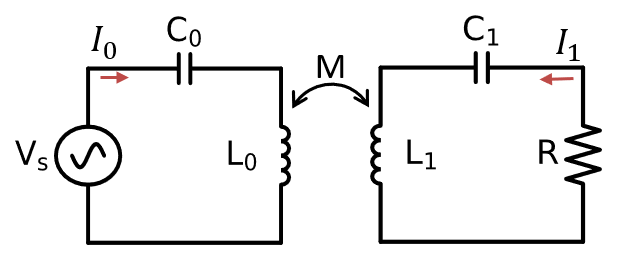
\includegraphics[width=0.7\linewidth]{images/2_ss_scheme.png}
    \begin{tikzpicture}[scale=1, every node/.style={scale=1}, american voltages]
        \draw
        (0,3.5) to [C, l=$C_1$, f_=$I_p$] (2.5,3.5)
        to [R, l=$r_1$, /tikz/circuitikz/bipoles/length=0.7 cm] (4,3.5)
        to [L, l=$L_1$] (4,0)
        to [short] (0,0)
        to [sI, l=$V_s$] (0,3.5);
        \draw
        (6,3.5) to [L, l_=$L_2$, mirror] (6,0)
        to [short] (10,0)
        to [R, l_=$R$] (10,3.5)        ;
        \draw (10,3.5) to [C, l_=$C_2$, f=$I_s$] (7.5,3.5)
        to [R,  l_=$r_2$, /tikz/circuitikz/bipoles/length=0.7 cm]
        (6,3.5);

        % source
        \node[below] at (5,3.5) {$M$};
        \draw [{<->}](4.234,2.6428) arc (139.9978:40:1);
        %  \draw [->,thick] (0,0.5) -- (0,3);
        %\node[below] at (0.5,2) {$V_p$};
        %\node[below] at (0.5,3) {+};
        %\node[below] at (0.5,0.5) {–};

        %  \draw [->,thick] (10,0.5) -- (10,3);
        %\node[below] at (10.5,2) {$V_s$};
        % \node[below] at (9.5,3) {+};
        % \node[below] at (9.5,0.5) {–};

    \end{tikzpicture}
    \caption{S-S structure.}
    \label{fig:ss topology}
\end{figure}

When the inductors and the capacitors in the resonance state, we have,
\begin{equation}
    \omega=\omega _0=\frac{1}{\sqrt{LC}},
    \label{formula:resonant frequency}
\end{equation}

where $\omega$ represents the working frequency, $\omega _0$ represents the resonant angular frequency of the circuit. Here, to maximize the transmission efficiency of the WPT system, we need to make the resonant frequencies of the primary side and secondary side consistent. Therefore,
\begin{equation}
    \omega _0 = \frac{1}{L_1C_1} = \frac{1}{L_2C_2}
\end{equation}

For any formed coil, we can measure its corresponding inductance value at a specified frequency. Thus, we can get the value of the compensation capacitor by formula \ref{formula:resonant frequency}.
\begin{equation}
    C = \frac{1}{\omega_0^2 L}
\end{equation}

% \begin{equation}
%     k=\frac{M}{\sqrt{L_1L_2}}
% \end{equation}
The compensation network of S-S structure is shown in figure \ref{fig:ss topology}.
The relationship between load voltage $V_R$ and power source voltage $V_s$ of SS topology shows below,
\begin{equation}
    V_R = \frac{j \omega MR}{(R+r_1)r_0 + \omega^2 M^2} V_s.
\end{equation}

% 传输效率计算的式子

\subsection{CLC-S compensation topology}

\begin{figure}[!t]
    \centering
    % 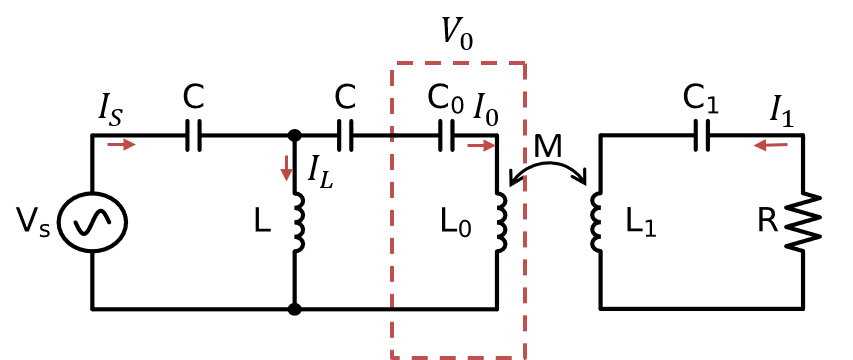
\includegraphics[width=0.93\linewidth]{images/2_clc_s_scheme.png}
    \resizebox*{\textwidth}{!}{
        \begin{tikzpicture}[scale=1, every node/.style={scale=1}, american voltages]
            \draw
            (-3.5,3.5) to [C, l=$C$, f_=$I_s$] (-0.5,3.5)
            to [C, l=$C$,f_=$I_1$] (1.5,3.5)
            to [C, l =$C_1$] (2.5,3.5)
            to [R, l=$r_1$, /tikz/circuitikz/bipoles/length=0.7 cm] (4,3.5)
            to [L, l=$L_1$] (4,0)
            to [short] (-3.5,0)
            to [sI, l=$V_s$] (-3.5,3.5);
            \draw(-0.5,3.5) to [L,l=$L$,f_=$I_L$] (-0.5,0);
            
            \draw
            (6,3.5) to [L, l_=$L_2$, mirror] (6,0)
            to [short] (10,0)
         to [R, l_=$R$] (10,3.5)        ;
            \draw (10,3.5) to [C, l_=$C_2$, f=$I_2$] (7.5,3.5)
            to [R,  l_=$r_2$, /tikz/circuitikz/bipoles/length=0.7 cm] 
            (6,3.5);
    
            % source
            \node[below] at (5,3.5) {$M$};
            \draw [{<->}](4.234,2.6428) arc (139.9978:40:1);
             \draw[line width=0.3mm,dashed,red](1.5,-0.5) rectangle(4.5,4.5);
        \node[above] at (3,4.5) {$V_1$};
        \end{tikzpicture}
    }
    \caption{CLC-S structure.}
    \label{fig:clcs topology}
\end{figure}

The compensation network of CLC-S structure is shown as in figure \ref{fig:clcs topology}.
According to the Kirchhoff's circuit laws we can get the following equation.

\begin{equation}
    \begin{align}
        V_S & = -jX_CI_S + j X_{L}I_L                      \\
        V_0 & = (-jX_{C_0}+jX_{L_0}+r_0)I_0 + j\omega MI_1 \\
        V_R & = j\omega I_0 +(-jX_{C_1}+jX_{L_1}+r_1)I_1   \\
        V_R & = -RI_1                                      \\
        I_S & = I_L+I_0
    \end{align}
\end{equation}

The relationship between load voltage $V_R$ and power source voltage $V_s$ of CLC topology shows below,
\begin{equation}
    V_R = - \frac{R}{R+r_1}\cdot \frac{\omega M}{X_L}V_S.
\end{equation}

\section{Underwater WPT system model}

% 海水环境下,海水作为传输介质其电气参数与空气中的相比有很大的区别,如表所示。因此,如式与式的常规互感模型无法反映出海水介质对传输的影响,不能完全、准确地描述海水下的传输行为。
In the seawater environment, the electrical parameters of seawater as the transmission medium are quite different from those in the air, as shown in the table \ref{table:permittivity}.
\begin{table}[!b]
    \centering
    \caption{The dielectric constant \& conductivity of some materials at 25$^\circ$C under 1kHz \cite{Wikipedia2020, Lenntech2021}.}
    \begin{tabular}{ |c|c|c|m{3.5cm}<{\centering}|m{3.5cm}<{\centering}| }
        % \thickhline
        \hline
        \textbf{Material} & \textbf{Relative permittivity} & \textbf{Conductivity}    \\\hline
        % \thickhline
        Vacuum            & 1                              & 0 S/m                    \\ \hline
        Air               & 1.0006                         & 0 S/m                    \\ \hline
        Ultra pure water  & 81                             & $5.5 \times 10^{-6}$ S/m \\ \hline
        Drinking water    & 81                             & 0.005 – 0.05 S/m         \\ \hline
        Seawater          & 81                             & 5 S/m                    \\ \hline
    \end{tabular}
    \label{table:permittivity}
\end{table}

It can be seen from table \ref{table:permittivity} that the relative permittivity of seawater is larger than that of air medium, resulting in a distributed capacitance between two conductors that are relatively close in seawater; at the same time, seawater has a certain conductivity , This is equivalent to connecting an eddy current loss resistor in series at both ends of the coil. Eddy current loss resistance and distributed capacitance will affect the impedance of the coil and generate additional power loss. Therefore, the conventional mutual inductance model of formula \ref{formula: basic VI matrix formula}. cannot reflect the influence of seawater media on transmission, and cannot completely and accurately describe the transmission behavior under seawater.

% 电路图

\begin{figure}[!t]
    \centering
    \resizebox*{.7\textwidth}{!}{
        \begin{tikzpicture} [scale=1, every node/.style={scale=1}, american voltages]

            \draw
            (0,6) to [R, l_=$R_{sea}$, o-] (3,6) to (4,6)
            to [R, l=$R$] (4,3)
            to [L, l=$L$] (4,0)
            to [short, -o] (0,0);
            \draw (3,6) to [C, l_=$C_{sea}$] (3,0);

            \node[single arrow,draw=black,fill=black!10,minimum height=2.5cm,shape border rotate=0] at (6,3) {};

            \draw
            (8,6) to [short, o-] (9.5,6)
            to [R, l=$R_{eq}$] (9.5,3)
            to [L, l=$L_{eq}$] (9.5,0)
            to [short, -o] (8,0);

        \end{tikzpicture}
    }
    \caption{Equivalent circuit of the coil under seawater.}
    \label{fig:coil under seawater}
\end{figure}

As shown in figure \ref{fig:coil under seawater}, $R_{sea}$ is the eddy current loss resistance, $C_{sea}$ is the distributed capacitance, both of which increase with the increase of operating frequency, $R$ is the internal resistance of the coil itself, and $L$ is the coil inductance. The mathematical expressions of equivalent inductance $L_{eq}$ and equivalent resistance $R_{eq}$ are as follows,

\begin{equation}
    L_{eq} = \frac{L-\omega ^2 L^2C_{sea}- C_{sea}R^2}{(1-\omega ^2 LC_{sea})^2 + \omega^2C_{sea}^2R^2},
    \label{formula: Leq}
\end{equation}
and
\begin{equation}
    R_{eq} = R_{sea} + \frac{R}{(1-\omega^2LC_{sea})^2+\omega^2C_{sea}^2R^2}.
    \label{formula: Req}
\end{equation}

Where $\omega$ is the operating angular frequency. Generally speaking, eddy current loss resistance $R_{sea}$ and distributed capacitance $C_{sea}$ are affected by many factors and are difficult to measure. Therefore, equations \ref{formula: Leq} and \ref{formula: Req} are not easy to calculate, and they are usually obtained with three-dimensional electromagnetic field simulation software or experiments. Since $R_{eq}$ is generally larger at high frequencies, underwater magnetic coupling resonance wireless energy transmission generally uses a working frequency below 1 MHz.